
\subsection{Feeding CPG Model}
For our analysis of sequence interval variability we used the CPG model developed by Vavoulis et al. \cite{Vavoulis2007}. The model describes the activity of  three neurons conforming the CPG feeding system of the mollusk \textit{Lymnaea} (N1M, N2v and N3t cells) along with the modulator neuron SO, which has a key role in the CPG activity by regulating the feeding cycle duration. Each CPG neuron is associated to one specific movement in the feeding activity: protraction (N1M), rasp (N2v) and swallow (N3t) \cite{Benjamin2012}. During protraction, the buccal mass and radular move forwards on the food. During rasp, the radular begins to move back to get the food into the buccal cavity. During swallow, the mouth closes and the radular pushes the food into the esophagus.

The dynamics of the single neuron models are based on a Hodgkin-Huxley conductance-based formalism \cite{HODGKIN1952} describing active ionic channels with specific features to reproduce the observed waveform from experimental recordings in each cell.
The Vavoulis et al. description of the individual neurons considers a two-compartment model to represent the soma and the axon as  differentiated structures coupled by an axial resistance \cite{Vavoulis2007}. This separation of the soma and the axon is used to regulate the interaction between the fast and slow dynamics in the model. The slow dynamics are located the soma, whereas the fast dynamics are included in the axon compartment of the model. This distributed formalism is represented in Fig. \ref{fig:2 compartments}, where each circle represents either soma or axon, with a distinct ionic current distribution. The description of the compartment dynamics is provided by equations (\ref{eq:soma}) and (\ref{eq:axon}) for soma and axon, respectively: 
%Cambios
%being \(i_X\) a different channel for each neuron in the CPG (N1M,N2v,N3t).

% which is usually represented in models as \(i_{e1} = g * (V_1 - V_2)\), where $V_1$ and $V_2$ represent the voltage in each of the two compartments and $g$ is the coupling conductance, the inverse of the axial resistance and $i_{e1}$ is the current that flows into one compartment from the other.
\begin{equation}
    \tau_m\frac{dV_S}{dt} = i_{inj} - i_{L,S} - i_X - i_{ec,S} - i_{syn} \\,
    \quad with \quad i_X = [i_{ACh},i_{NaL},i_T]
    \label{eq:soma}
\end{equation}

\begin{equation}
    \tau_m\frac{dV_A}{dt} = -i_{L,A} - i_{NaT} - i_K - i_{ec,A}
    \label{eq:axon}
\end{equation}

\begin{figure}
\centering
\begin{subfigure}[t]{0.5\textwidth}
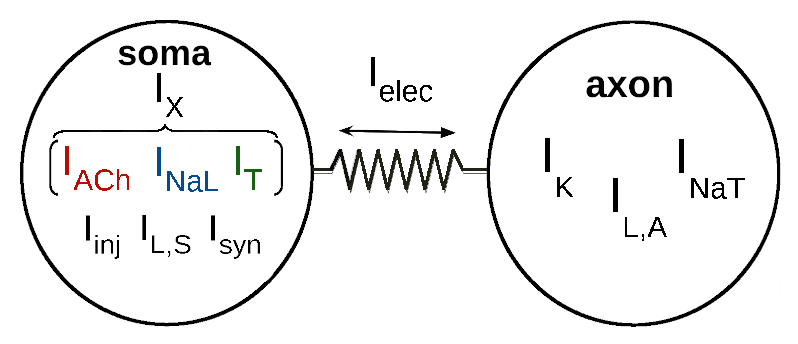
\includegraphics[width=\textwidth]{img/methods-paper-modelo/figure1a.eps} 

\caption{} \label{fig:2 compartments}
\end{subfigure}
\hfill
\begin{subfigure}[t]{0.49\textwidth}
\centering
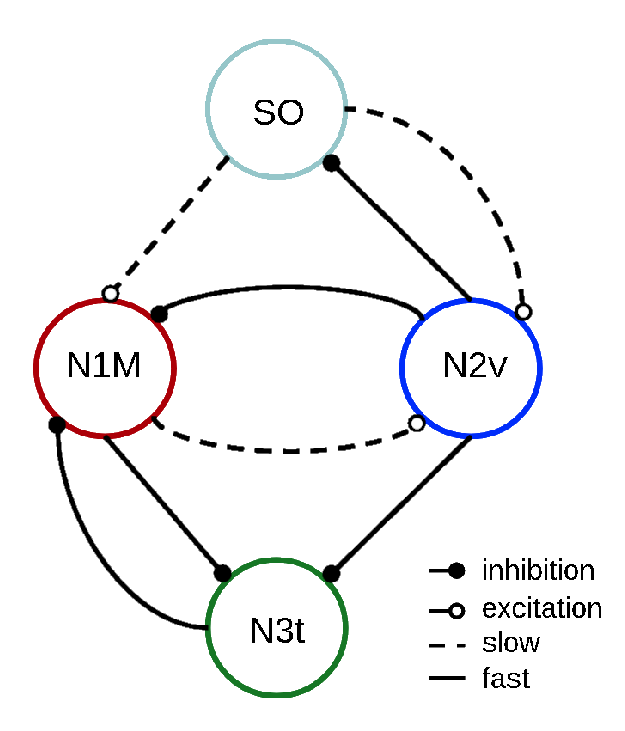
\includegraphics[width=\textwidth]{img/methods-paper-modelo/figure1b.eps} 
%TODO FIX
\caption{} \label{fig:CPG diagram}
\end{subfigure}
 
 \caption{\textbf{Panel (a)}. Ionic channel distribution in the two-compartment description for the individual neurons in the Vavoulis et al. model \cite{Vavoulis2007} used in this study. At the soma: $I_{ACh}$, acetylcholine ionic channel; $I_{NaL}$, slowly inactivating sodium ionic channel;$I_T$, low-threshold calcium current; $I_{inj}$, injected current; $I_{L,S}$, leakage current in the soma; $I_{syn}$, synaptic current. At the axon: $I_{NaT}$, fast inactivating sodium current; $I_K$, delayed rectifier potassium current; $I_{L,A}$, leakage current in the axon. The electrical couplings are described as $I_{ec,S}=g_{ec}(V_S-V_A)$ and $I_{ec,A}=g_{ec}(V_A-V_S)$, respectively, being $g_{ec}$ the coupling conductance. The color for each $I_X$ current represents the CPG neuron that includes it at the soma,  N1M, N2v and N3t, respectively, as shown in panel (b). \textbf{Panel (b)}. Connection scheme for the {\sl Lymnaea} feeding CPG circuit model. For details on the ionic channel current descriptions and associated parameters, see \cite{Vavoulis2007}. The colors indicating each neuron in the circuit match those in the representation of their corresponding somatic membrane potential traces throughout the paper. 
}
    
    % \label{fig:2 compartments}
\end{figure}


\vspace{0.3in}

\noindent Here we follow the notation of~\cite{Vavoulis2007} where $\tau_m$ represents the time constant of the membrane (in ms) given by the ratio of the membrane capacitance (in nF) and the leakage conductance (in $\mu$S).  In equations (1) and (2), $i$ variables (given in mV) are the product of the corresponding currents (in nA) times the passive input resistance given in M$\Omega$.
%, $i=I*R$, where  $R$ is given in M$\Omega$.
% Añadir explicación de unidades********. 


The soma compartment contains a slow current $I_X$ whose ionic nature depends on the specific CPG neuron described (see Fig.~\ref{fig:2 compartments}). Thus, $I_X$  represents one channel, either $I_{ACh}$, $I_{NaL}$ or $I_{T}$, responsible of the specific slow dynamics associated with neurons N1M, N2v and N3t, respectively.  Along with the slow ionic channel and the leakage channel  $I_{L,S}$, the soma compartment also receives the synaptic current $I_{syn}$ and the injection current $I_{inj}$. All currents are explained in detail below.
%TODO al final Leakage no se pone aqui?

%A more extended explanation of these channels and the property they produce is . Along with this slow activation channels, there are also found in the soma $i_{inj}$, an injected current, and $i_{syn}$ a synaptic input that is widely explained below. These are also represented in figure \ref{fig:2 compartments}

On the other hand, fast channels are part of the axon compartment: a fast inactivating sodium current $I_{NaT}$ and a delayed rectifier potassium current $I_{K}$. These channels, along with the axon leakage channel  $I_{L,A}$ are also represented in Fig.~\ref{fig:2 compartments}, for their detailed description see~\cite{Vavoulis2007}. 


% ***Descripción breves de corrientes en terminos de cuales son lentas y rápidas con referencia a la Fig.1
% y la i_x

The model cells as described above are not endogenously bursters. To achieve a realistic bursting activity in each neuron, a distinct constant value of  \(i_{inj}\) is applied to the cells. %  Values of \(i_{inj}\) used in this study to obtain realistic bursting activity. 
%TODO añadir " in the circuit".

 The CPG topology scheme is shown in Fig. \ref{fig:CPG diagram}, where the connections between neurons are represented by dashed or solid lines, depending on whether the connection is slow or fast, respectively, and filled or empty circles at their end denoting the direction and the effect on the postsynaptic neuron: excitation (empty circles) or inhibition (filled circles).
Individual neurons following the previous description are connected by graded synapses, defined by equations (\ref{eq:syn1}-\ref{eq:syn2}) \cite{Vavoulis2007}:

% \begin{equation}
%     i_{syn} = \sum_j \gamma_{syn,j} s_j (V_S - E_{syn,j})
%   \label{eq:syn1}
% \end{equation}
% % TODO FIX
% \begin{equation}
%     \frac{ds_j}{dt} = \frac{r_{j}-s_j}{\tau_{syn,j}}
% \end{equation}

% \begin{equation}
%   \frac{dr_j}{dt} = \frac{r_{\infty,j}-r_j}{\tau_{syn,j}}
% \end{equation}

% \begin{equation}
%     r_{\infty,j}=\frac{1}{1+e^{(-40-V_{pre_{V_S}})/2.5}}
%      \label{eq:syn2}
% \end{equation}


\noindent where index $j$ runs over all presynaptic neurons and \(\gamma_{syn,j}, E_{syn,j},\tau_{syn},V_{pre_{V_S}}\) are the product of input resistance and maximal synaptic conductance, the synaptic reversal potential, the synaptic time constant and the presynaptic potential, respectively.
%cambio

Together with the effect of the distinct connections conforming the circuit, the neuron dynamics in this model is shaped by the ionic channels at each cell and their associated parameters. The resulting triphasic CPG rhythm with distinct voltage waveforms of spiking-bursting activity is displayed in Fig. \ref{fig:model simulation}, where the effect of the connections in building the phase between neurons can also be observed. The traces correspond to a simulation of the complete circuit model, i.e., all connections shown in Fig. \ref{fig:CPG diagram} are active. 


\begin{figure}[h!]
    \centering
    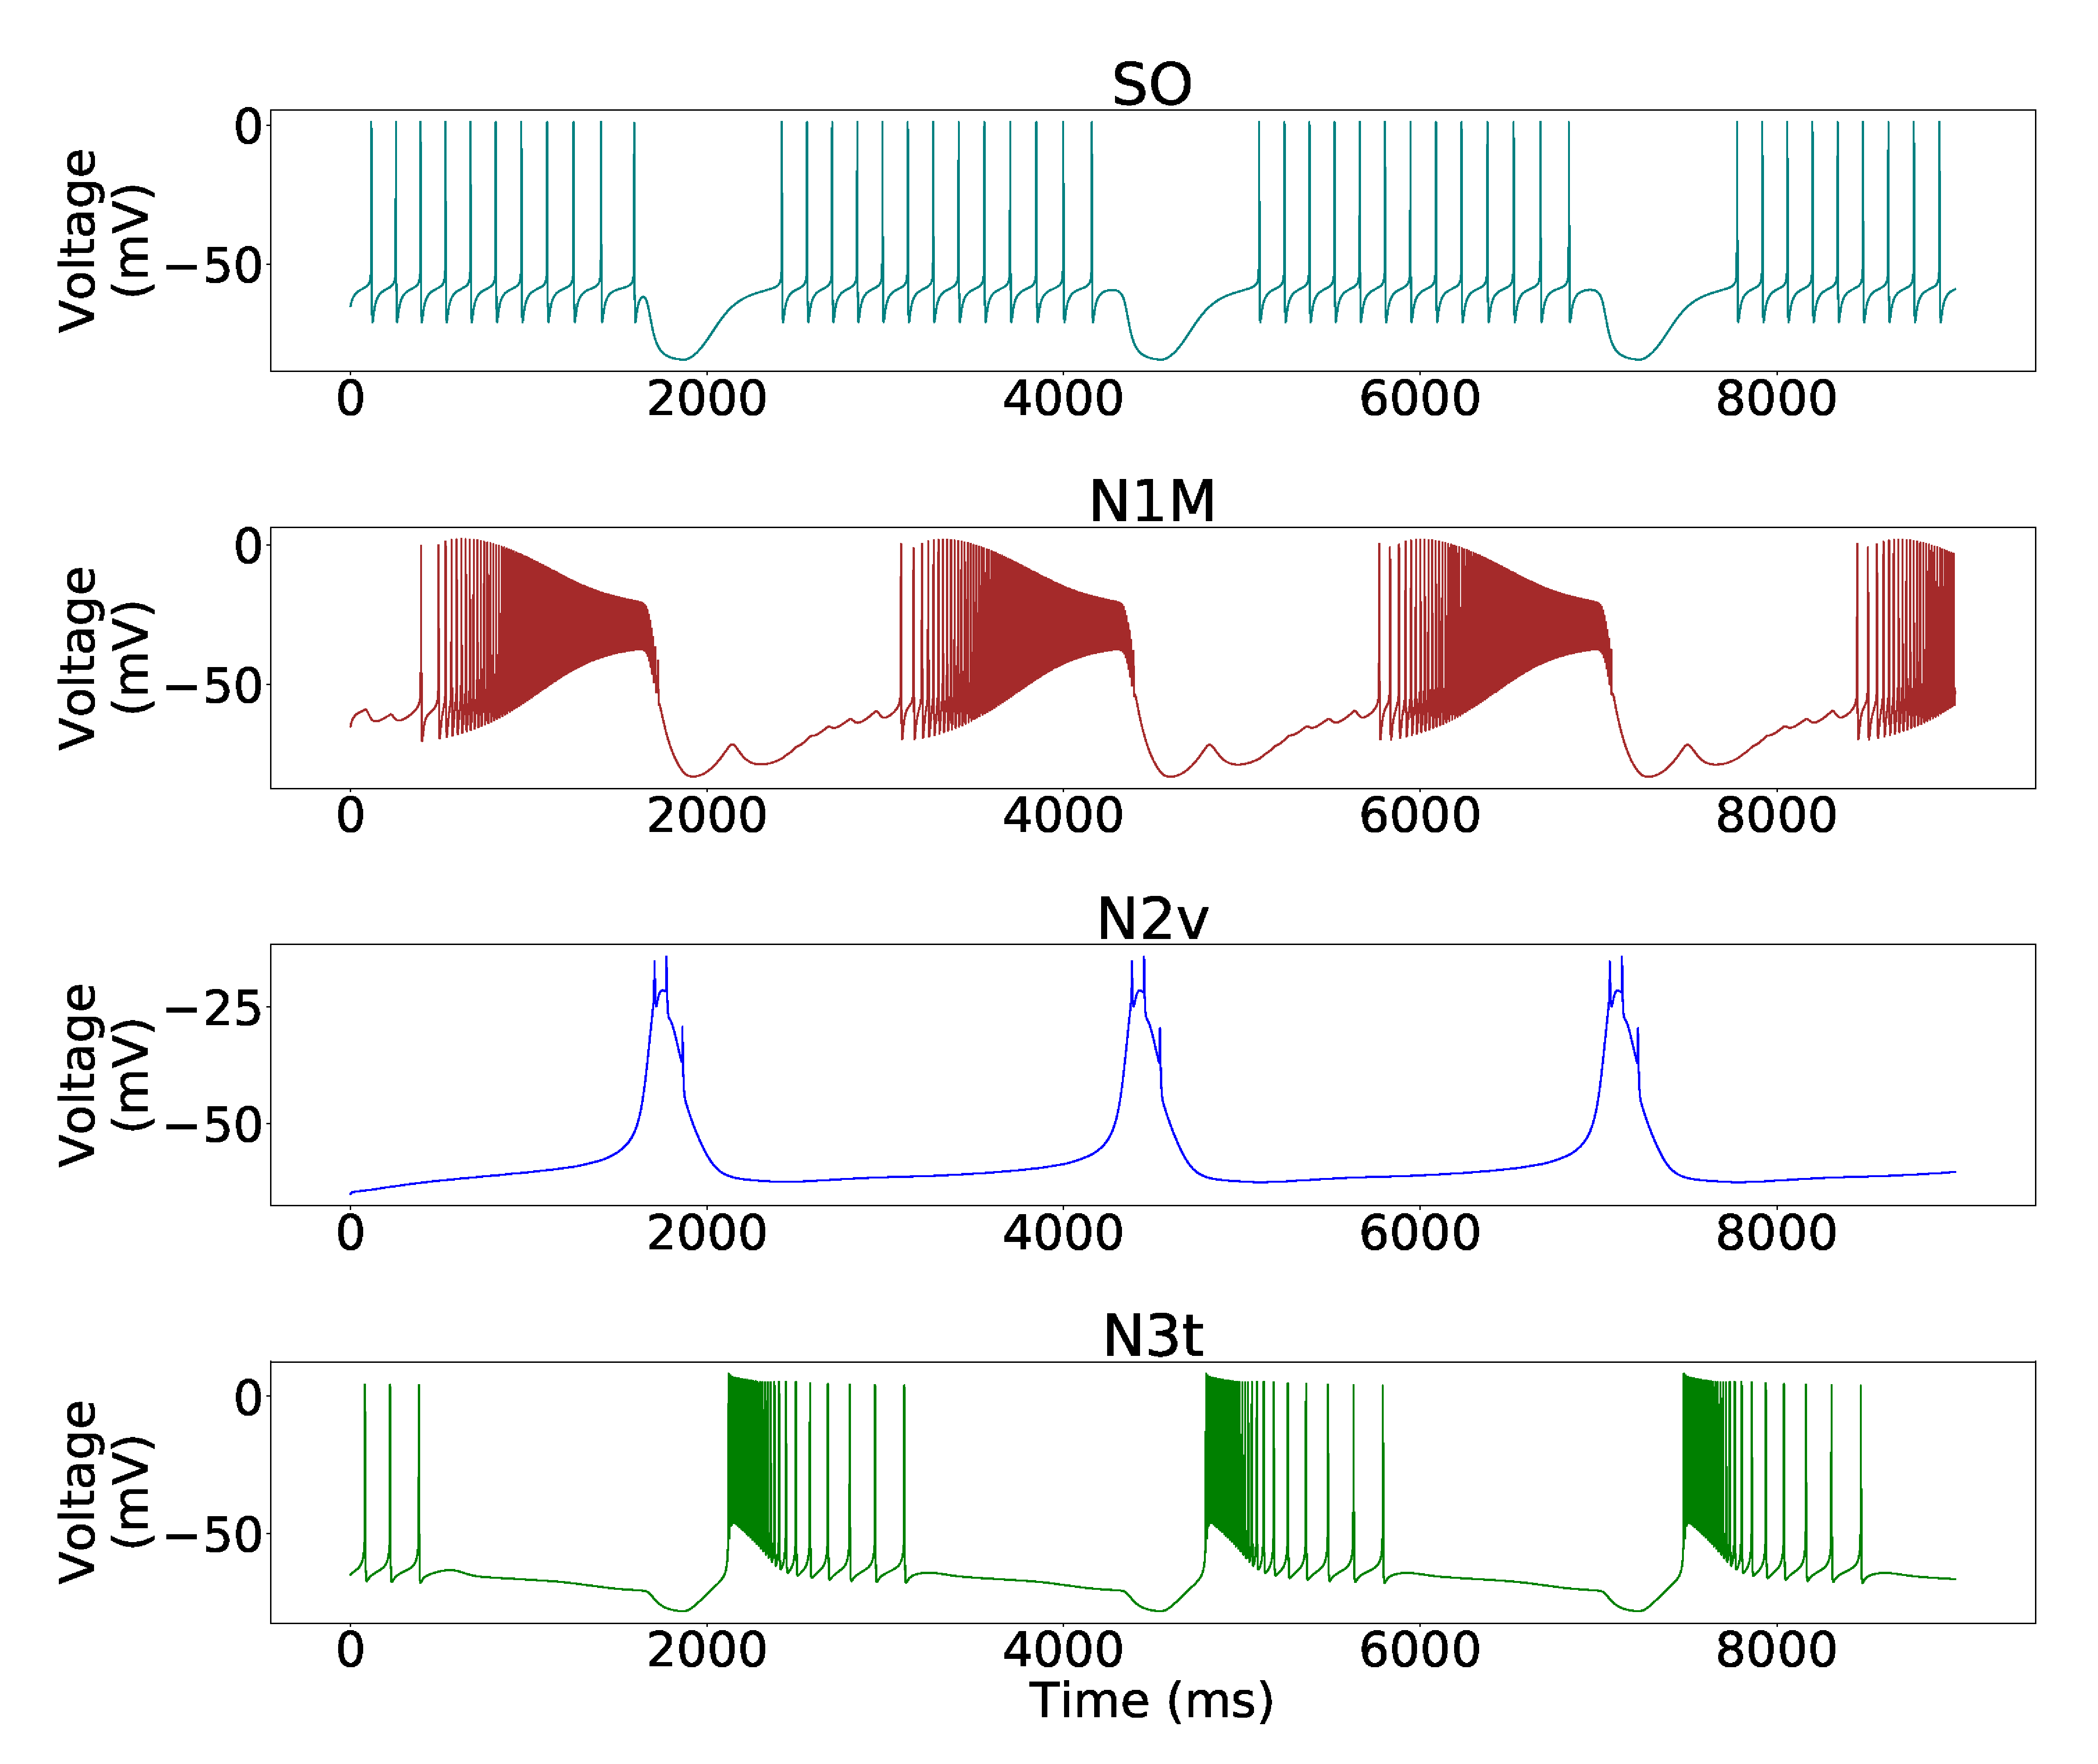
\includegraphics[width=\linewidth]{img/methods-paper-modelo/figure2.eps}
    \caption{Triphasic feeding rhythm as produced by the circuit CPG model described in Fig. \ref{fig:CPG diagram}. In this simulation, $i_{inj}$ values applied to each neuron are 8.5, 6, 2 and 0 mV, respectively.}
    \label{fig:model simulation}
\end{figure}

The distinct waveforms for each neuron are mainly due to their specific ionic channel dynamics. On the one hand, N1M voltage characteristics are provided by an acetylcholine sensitive channel (\(i_{ACh} = 200 * p^3 * (V_S + 30)\)), which causes the gradual spiking frequency increase as well as the visible plateau, i.e., the slow wave is sustained before hyperpolarization. On the other hand, N2v has a slowly inactivating sodium channel (\(i_{NaL} = 2 * p^3 * q^3 * (V_S-55)\)), which causes the slow depolarization in this neuron. N2v neuron has a lower spiking frequency caused by the conductance value given for the axial $g_{ec}$ linking the two compartments, which is much lower in this cell. Finally, the N3t neuron has the particularity of a post inhibitory rebound, which generates an initial fast spiking followed by a decrease in the firing rate as the burst evolves. This latter property is caused by a low-threshold calcium channel (\( i_T = 3.27 * p^3 * q *(V_S-80)\)).

%cambios
In contrast to the N1M, N2v and N3t neurons of the CPG, the model of the SO neuron has no \(I_X\) channel, so its activity is the result of the combination of the common ionic channels in the axon and the soma.
% ****no se dice nada de la SO ****

\subsection{Inducing variability by current injection}
\label{subsec:inj protocol}
The spiking-bursting activity of the model CPG neurons can be modulated by using an additional current injection on each cell, implemented in the \(i_{inj}\) term of equation (\ref{eq:soma}), as performed in many experimental protocols. Depending on the value % of the current 
applied,%TODO current o value applied?
% the corresponding neuron dynamics changes. While for N2v a change in this current injection corresponds to a change in burst frequency (i.e. the number of bursts increases/decreases), for the rest of the neurons in the model (N1M, N3t and SO) a change in \(i_{inj}\) affects their burst duration. %%TODO ????
the corresponding neuron dynamics changes. While for N2v a change in this injection corresponds to a change in burst frequency (i.e. the number of bursts increases/decreases),
for the rest of the neurons in the model a change in \(i_{inj}\) affects burst duration for N3t and SO,  and the length of the depolarization phase in N1M.


Whilst the single neuron model descriptions have no intrinsic variability, the effect produced by the modulation of the injected current in each neuron induces variability into the circuit, which allows characterizing the sequence intervals and the period, the associated robustness of the rhythm and the presence of dynamical invariants. Such stimulation has been used previously in the living circuit, as reported by Elliot et al. \cite{Elliott1991}. The authors of this work showed that it is possible to activate the feeding CPG with variability caused by current injection into individual cells in the circuit. CPG rhythms obtained under this type of stimulation differ depending on which neuron is being stimulated. 

% Even though this CPG model do not present intrinsic variability, thanks to the current \(i_{inj}\), variability is induced into the model, effectively changing burst duration. This current injection has also been used in Lymnaea preparation in living elements, stimulating N1M and SO, obtaining rhythm. Neural sequences obtained after the stimulation differ one another depending on which neuron is being stimulated. 

By varying the current injected into N1M, its burst duration is kept nearly constant, but its depolarization phase before the spiking activity begins becomes longer. Since N3t is the neuron fitting in the sequence in that phase (see Fig. \ref{fig:model simulation}), it also increases its burst duration, being the most variable one in the CPG rhythm. 

When %current 
value \(i_{inj}\) is increased on neuron SO, its burst duration becomes longer. Since SO has a modulator effect over N3t and N1M, it also alters the burst duration of these two neurons.

Neuron N3t also shows variable burst duration when an evolving current is injected. When \(i_{inj}\) increases on N3t, its burst duration increases, elongating the N1M depolarization phase.  

Finally, when current is applied to N2v the effect on its burst duration or the burst duration of the rest of the neurons is rather small. However, \(i_{inj}\) % current 
modulates N2v burst frequency through the hyperpolarization phase. 

%cambios
Therefore, we used a current ramp protocol to induce variability in the CPG model defined as follows: a ramp variable $c$, which controlled the current injection value ($i_{inj}=c$) %TODO
on the neuron being stimulated, was increased from a minimum to a maximum value, and then decreased back to the initial value. This was repeated twice in each simulation. The ramp variable was modified with a fixed step value every 4.6 seconds (the approximate duration of two N3t bursts).
% occurrence of each two bursts in N3t neuron (every 5 seconds). ***discutimos esto, es cada burst o cada dos como dice abajo, quizás convendría decir que corresponde a ese tiempo en el modelo sin estímulo. Por otro lado el lector se podría preguntar por qué no es una rampa de subida y bajada prestablecida en el tiempo***
The minimum and maximum $c$ values were different in each cell and were %chosen experimentally using model simulations 
tuned to generate realistic spiking-bursting behavior. %cambios : añadir por si experimentally no se entiende bien? depending on the effect of the injected current on the neuron to ensure robust burst generation in all neurons 
%Note that this variable $c$ value which goes through the different values in the ramp is $i_{inj}$ value, replacing the constant value of this current.
All parameters used for the simulation analyses reported in this paper are summarized in Table \ref{table:inj values}. An example of how this ramp current injection affects the rhythm is shown in Fig. \ref{fig:complete ramp example}. 
%cambios : quitar esta frase e indicarlo en seccion 2.3
% The rest of model and synapse parameters used to simulate the model are the same ones specified in the paper that describes the Vavoulis et al. model \cite{Vavoulis2007}.


\begin{table}[h!]
\centering
\begin{tabular}{c|cccc|c|ccc|}
\multirow{2}{*}{\textbf{\begin{tabular}[c]{@{}c@{}}Neuron\\ stimulated\end{tabular}}} & \multicolumn{4}{c|}{\textbf{\(i_{inj}\) value}}                 & \multirow{6}{*}{} & \multicolumn{3}{c|}{\textbf{Ramp values ($c$)}}   \\ \cline{2-5} \cline{7-9} 
                                                                                      & \textbf{SO} & \textbf{N1M} & \textbf{N2v} & \textbf{N3t} &                   & \textbf{Min} & \textbf{Max} & \textbf{Step} \\ \cline{1-5} \cline{7-9} 
\textbf{N1M}                                                                          & 8.5         & $c$            & 2            & 0            &                   & 0            & 10.5         & 0.5           \\ \cline{1-5} \cline{7-9} 
\textbf{N3t}                                                                          & 9           & 10           & 1            & $c$            &                   & 0            & 5            & 0.25          \\ \cline{1-5} \cline{7-9} 
\textbf{SO}                                                                           & $c$           & 10           & 1            & 4            &                   & 8.2          & 13           & 0.25          \\ \cline{1-5} \cline{7-9} 
\end{tabular}
\caption{List of \(i_{inj}\) values that yield realistic bursting rhythms for each neuron in the model CPG used in the stimulation protocols reported in this paper. The left section of the table displays the \(i_{inj}\) values applied to each neuron (columns) during each simulation condition (rows). Ramp values on the right section refer to the minimum and maximum values of the ramp variable $c$ in each simulation, increasing \(i_{inj}\) in the specified step every 4.6 seconds (the approximate duration of two N3t burst) to induce variability.} \label{table:inj values}
\end{table}


\begin{figure}[h!]
    \centering
    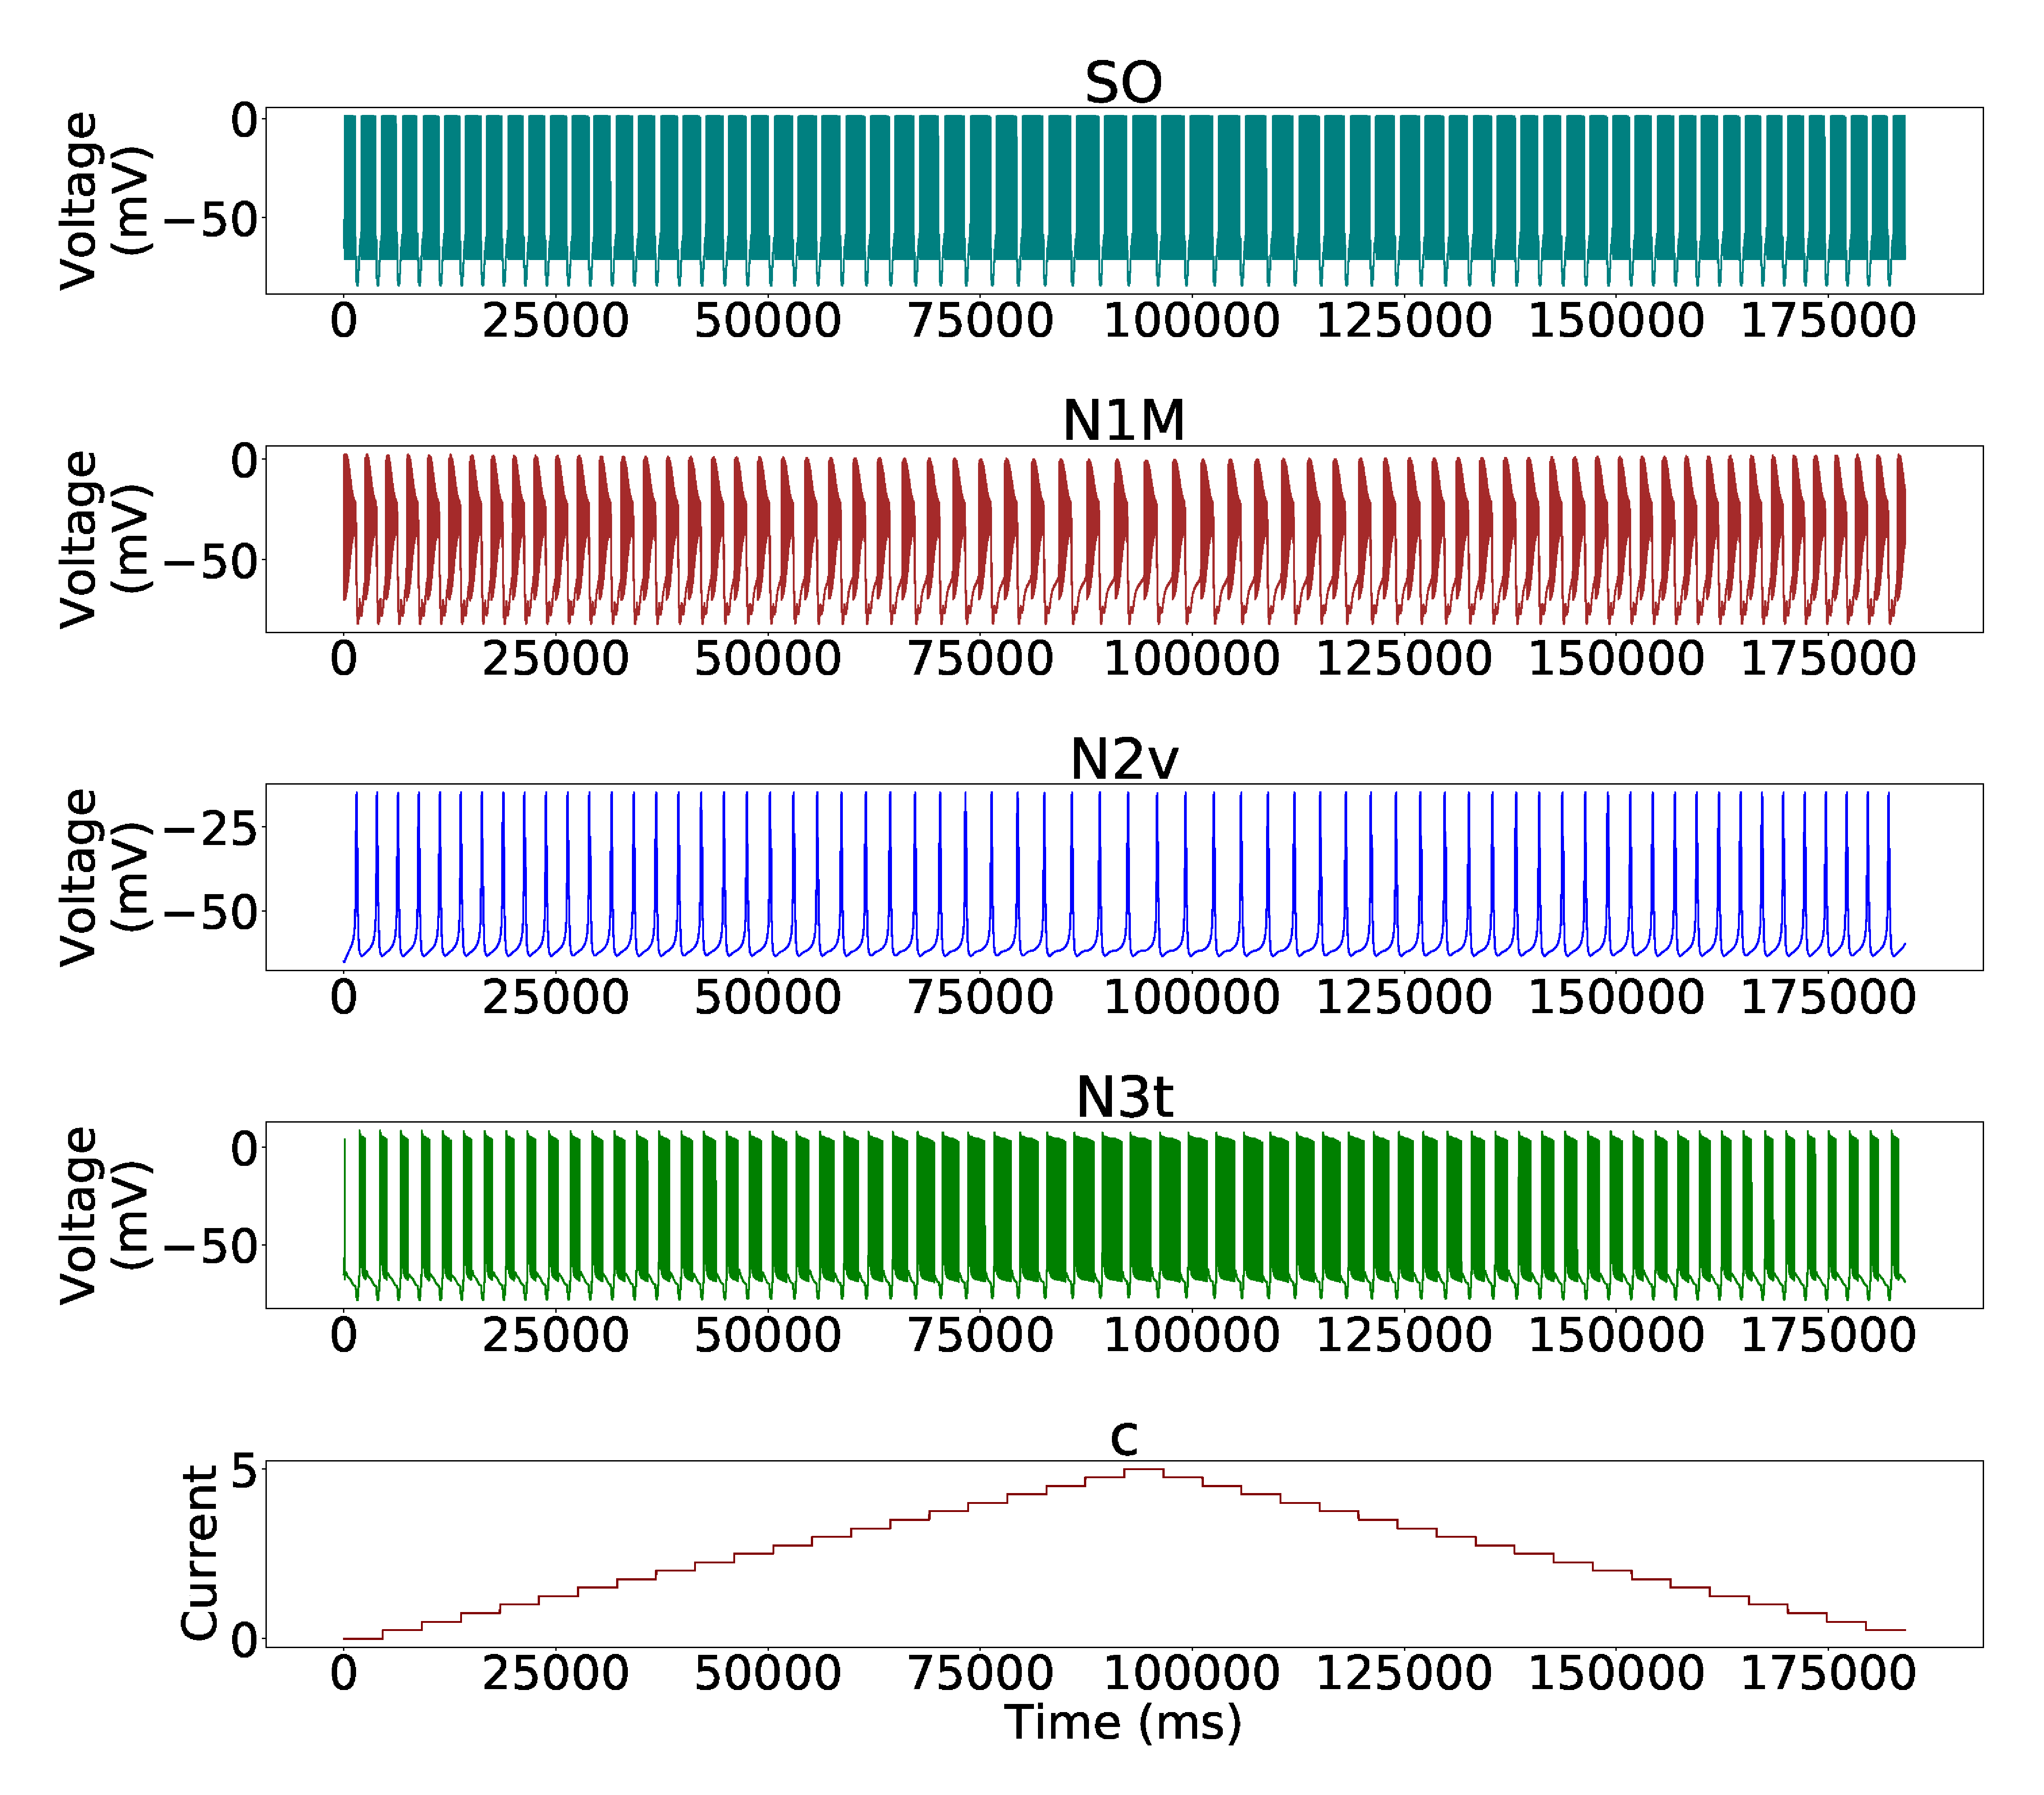
\includegraphics[width=\textwidth]{img/methods-paper-modelo/figure3.eps}
    \caption{Illustration of the CPG activity when a current ramp \(i_{inj}\) is applied to N3t. Variability in the sequence intervals was induced by applying two consecutive ramps as the one shown in this figure into different cells.  }
    \label{fig:complete ramp example}
\end{figure}


\subsection{Model simulation specifications and statistical analysis}
Simulations of the Vavoulis et al. model \cite{Vavoulis2007} were implemented in C++. The code of the feeding CPG model implementation is available at \url{https://github.com/GNB-UAM/CPG-feeding-Lymnaea}. Each simulation had the duration of two consecutive cycles of up and down ramps as the one shown in Fig. \ref{fig:complete ramp example} using the parameters described in Table \ref{table:inj values}. The number of bursts in each simulation was approximately 140 (this number slightly depends on the neuron stimulated). Parameter values such as reversal potentials and synaptic conductances were the same ones specified in \cite{Vavoulis2007}.
The statistical analysis was done in Python 3.6. For the temporal variability study, first the spikes were detected %\sout{using a threshold protocol. Due to the drift in the spike amplitude during the bursting of some of the neurons (as N2v), the spike detection was performed over the $1^{st}$ derivative of the signal}
using the change in the derivative during the computation of the model along with a threshold condition. Then, bursts were identified from the temporal structure of the spikes, and intervals were characterized by the timing of the first and last spike in each burst. 

Thus, all intervals defined below in section \ref{subsec:intervals} were measured and their variability was characterized by statistical analysis tools, i.e,  boxplots and linear correlations. For the boxplots, the Python library matplotlib.pyplot used each cycle-by-cycle interval duration. Linear regression from sklearn Python library was used to quantify the relation of the sequence intervals to the instantaneous period of each cycle. 

\subsection{Time references, intervals and CPG sequence}
\label{subsec:intervals}
The variability study addressed here is based on the characterization of  cycle-by-cycle intervals in the rhythm produced by the model CPG. % In order to explore possible dynamical invariants on this \textit{Lymnaea} feeding CPG, the intervals here analyzed follow the ones defined for the stomatogastric CPG dynamical invariants \cite{Elices2019}. Hence, based on the burst duration we will have in each cycle all corresponding burst duration intervals and some derived intervals obtained by the combination of pair of neurons, as well as the period. The resulting intervals here analyzed are shown in figure \ref{fig:intervals}. 
In our analysis of variability, we assess the presence of linear relationships between the intervals that build the sequence and the cycle-by-cycle period to characterize and unveil similar dynamical invariants as those found in the stomatogastric CPG \cite{Elices2019}. 
%Hence, we characterize the intervals building the CPG sequence, including its period. 
%on the burst duration we will have in each cycle all corresponding burst duration intervals and some derived intervals obtained by their combination of pair of neurons, including the period.
% Hence, the burst events detected are going to be used to define three intervals in the trace of each individual neuron, and two additional intervals defined from the relation between two neurons. 
This is illustrated in Fig. \ref{fig:intervals}, where single neuron intervals and intervals defined between neurons are depicted. 
%cambios
The intervals here analyzed can be measured for any three neurons following a robust triphasic rhythm. In this paper N1, N2 and N3 represent the feeding CPG neurons simulated in the model: N1M, N2v and N3t, respectively.

% Here is the definition of each interval:
% \begin{enumerate}
%     \item \textbf{Burst Duration (BD)}, measured as the time interval between the first and the last spike of the burst (start to end in the trace of a given neuron).
%     \item \textbf{Inter burst interval (IBI)}, characterised as the difference between the last spike of a burst and the first one of the next one (end to start in the trace of a given neuron).
%     \item \textbf{Period}, which envelops the bursts from the three neurons, measured as the distance between the first spike of one burst in a neuron and the first spike of the next one on that neuron (start to start).
%     \item \textbf{NeuronX-NeuronY interval}, this interval is measured from the burst beginning of neuron X to the burst beginning of neuron Y (start X to start Y).
%     \item \textbf{NeuronX-NeuronY delay}, being the time lapse between the burst end of a neuron X and the burst beginning of neuron Y. (end X to start Y).
% \end{enumerate}

\begin{figure}
\centering
\begin{subfigure}[t]{\textwidth}
\centering
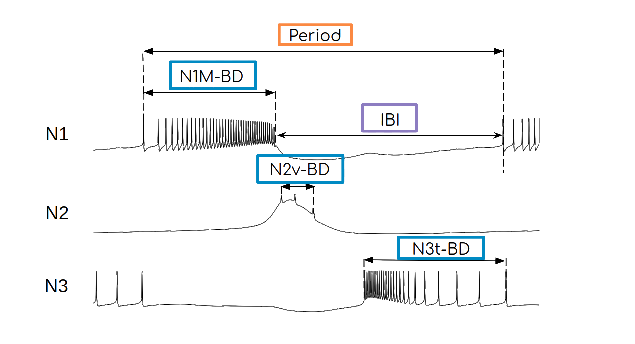
\includegraphics[scale=0.8]{img/methods-paper-modelo/figure4a.eps} 
\caption{} \label{fig:intervals_bd}
\end{subfigure}
% \hfill

    \vspace{1cm}
\begin{subfigure}[t]{\textwidth}
\centering
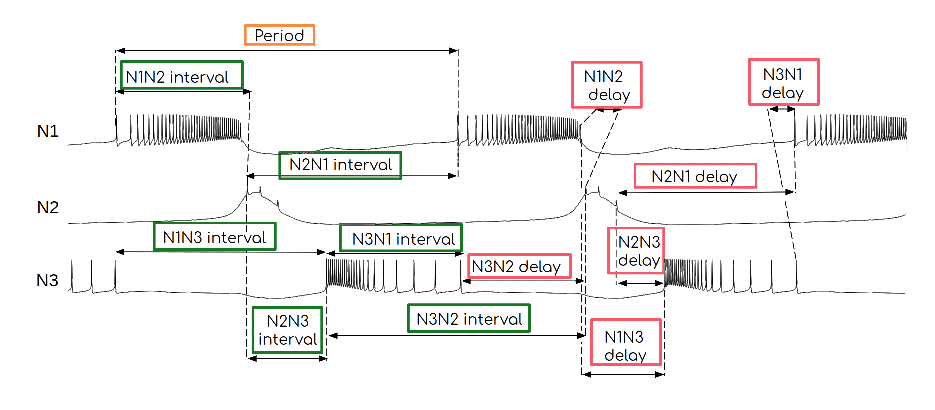
\includegraphics[scale=0.8]{img/methods-paper-modelo/figure4b.eps} 
\caption{} \label{fig:intervals_der}
\end{subfigure}
 
 \caption{\textbf{Panel A}. Individual neuron sequence interval definitions. Each BD label represents the burst duration, defined as the time interval from the first spike to the last spike in the neuron's burst. Period was measured as the interval from the first spike of N1 burst to the first spike of the next N1 burst, covering three phases %(N1M,N2v, N3t) 
 in relation to the activity of the other neurons. IBI represents the interburst interval, defined as the time from the last spike of a neuron's burst to the first one of the next burst in the same neuron.
    \textbf{Panel B}. Definition of intervals involving pairs of neurons. NXNY interval represents interval from NX start to NY start. NXNY delay represents interval from NX end to NY start. Period was measured from N1 start to N1 start, covering the three phases of the CPG rhythm.
    }
    
    \label{fig:intervals}
\end{figure}

\clearpage
\newpage



% ***quizás convendría añadir una subsección en los métodos diciendo cuál es la duración de las series temporales, las ráfagas que contienen y que se detectan los spikes para caracterizar los intervalos ciclo a ciclo. También que la variabilidad se caracerizó con boxplots del coeficiente de variación de todos los intervalos. Las figuras de los boxplots no parecen en porcentajes, los valores negativos habría que explicarlos en términos de que la fase de algunas neuroans se adelanta con respecto a lo definido en la figura 4 ***
